
\documentclass[landscape, DIV=99, 14pt]{scrartcl}

\renewcommand*{\familydefault}{\sfdefault}

\RequirePackage{graphicx}
\RequirePackage[utf8]{inputenc}
\RequirePackage{hyperref}
\RequirePackage[gen]{eurosym}
\RequirePackage{multirow}
\RequirePackage{booktabs}
\RequirePackage[table]{xcolor}
\RequirePackage{siunitx}
\RequirePackage{etoolbox}
\RequirePackage{etoolbox}

\setlength{\parindent}{0cm}

\robustify\bfseries
\robustify\itshape

\begin{document}
\sisetup{detect-all = true}

\twocolumn
\section*{Zusammenfassung BMW Kosten}
\null
\vspace{1cm}
\begin{center}
%                           trim={<left> <lower> <right> <upper>}
\includegraphics[width=10cm, trim={4cm 0 4cm 5cm}]{images0/kosten_verteilung.png}
\end{center}

\includegraphics[width=1.4\columnwidth]{images0/kosten_maximus.png}

\pagebreak

\begin{itemize}
    \item Wertverlust
    \begin{itemize}
        \item Kaufpreis minus Verkaufspreis
    \end{itemize}
    \item Kraftstoffe
    \begin{itemize}
        \item Summe aller Tankstellenbesuche
    \end{itemize}
    \item Wartung und Reparatur
    \begin{itemize}
        \item Regul\"are Wartungsarbeiten (\"Olwechsel, etc)
        \item Reparaturen Aufgrund technischer Defekte
        \item Unfallsch\"aden
    \end{itemize}
    \item Versicherung
    \begin{itemize}
        \item J\"ahrlicher Versicherungsbeitrag
        \item Mobilit\"ats-Service
    \end{itemize}
    \item Steuern
    \begin{itemize}
            \item J\"ahrliche KFZ-Steuer
    \end{itemize}
\end{itemize}


\twocolumn

\section*{Tesla Model Y, neu, Strom, Kredit}
\begin{center}
\includegraphics[width=0.5\textheight]{images1/tesla-model-y-n514kS5-boundaries_.png}
\null
\vspace{0.5cm}
\includegraphics[width=0.5\textheight]{images1/tesla-model-y-n514kS5-calc_df_.png}
\end{center}

\pagebreak
\begin{center}
\includegraphics[width=0.9\columnwidth]{cars/tesla-model-y.jpg}

Tesla Model Y
\end{center}

\begin{itemize}
    \item LL/BJ: 0/2022, 5-Sitzer $\rightarrow$ Laufzeit: 7 Jahre
    \item \href{https://www.tesla.com/de_de/modely/design\#overview}{Weblink}
    \item \emph{Gesch\"atzter} Spritpreis \"uber Haltedauer: 0.31 \euro{}/kWh
    \item Antrieb: Strom, mit 514 PS
    \item Restwert nach Faustformel (Kaufpreis $\times$ 19.8\%): 11502.70 \euro{}
\end{itemize}

\begin{small}
\emph{Meinung Nataliya:} 8/10: Zu Teuer. Sehr viel Platz. Keine Stufe auf dem mittleren Platz. Automatisches Bremsen toll. Kofferraum groß genug. Display seltsam aufgeteilt. Display zu groß.
        
\emph{Meinung Grzegorz:} 8/10: Sehr bequemes, luxuri\"oses Auto. Viel Platz, viel Leistung, gro\ss{}e Reichweite. Schlechtes Kofferraum Management, Keine Hutablage, keine Sicherung unter dem Sitz.
\end{small}

\pagebreak


\twocolumn

\section*{Tesla Model 3, neu, Strom, Kredit}
\begin{center}
\includegraphics[width=0.5\textheight]{images1/tesla-model-3-n325kS5-boundaries_.png}
\null
\vspace{0.5cm}
\includegraphics[width=0.5\textheight]{images1/tesla-model-3-n325kS5-calc_df_.png}
\end{center}

\pagebreak
\begin{center}
\includegraphics[width=0.9\columnwidth]{cars/tesla-model-3.jpg}

Tesla Model 3
\end{center}

\begin{itemize}
    \item LL/BJ: 0/2022, 5-Sitzer $\rightarrow$ Laufzeit: 7 Jahre
    \item \href{https://www.tesla.com/de_de/model3/design\#overview}{Weblink}
    \item \emph{Gesch\"atzter} Spritpreis \"uber Haltedauer: 0.31 \euro{}/kWh
    \item Antrieb: Strom, mit 325 PS
    \item Restwert nach Faustformel (Kaufpreis $\times$ 19.8\%): 8724.75 \euro{}
\end{itemize}

\begin{small}
\emph{Meinung Nataliya:} 0/10: 
        
\emph{Meinung Grzegorz:} 0/10: 
\end{small}

\pagebreak


\twocolumn

\section*{Mazda 6, neu, Benzin, Kredit}
\begin{center}
\includegraphics[width=0.5\textheight]{images1/mazda-6-n192kB5-boundaries_.png}
\null
\vspace{0.5cm}
\includegraphics[width=0.5\textheight]{images1/mazda-6-n192kB5-calc_df_.png}
\end{center}

\pagebreak
\begin{center}
\includegraphics[width=0.9\columnwidth]{cars/mazda-6-neu.png}

Mazda 6
\end{center}

\begin{itemize}
    \item LL/BJ: 0/2022, 5-Sitzer $\rightarrow$ Laufzeit: 7 Jahre
    \item \href{https://konfigurator.meinauto.de/mazda/neuwagen/48-6/angebote/6-kombi/konfigurator/\#!/extras/exclusive-line/8846370/10,11/private/65352-5416-204698/984/61c9aa657e74c/cash-purchase/32545--287374/48,0,10000,0,0,0,0,0,}{Weblink}
    \item \emph{Gesch\"atzter} Spritpreis \"uber Haltedauer: 1.64 \euro{}/l
    \item Antrieb: Benzin, mit 192 PS
    \item Restwert nach Faustformel (Kaufpreis $\times$ 19.8\%): 6080.38 \euro{}
\end{itemize}

\begin{small}
\emph{Meinung Nataliya:} 6/10: Zu laut, stinkt, ruppelig, eng vorne und hinten. Navi etwas seltsam.
        
\emph{Meinung Grzegorz:} 4/10: Tolles Au\ss{}endesign, sehr sch\"oner Innenraum und gro\ss{}er Kofferaum. Motor schwach und klapprig, Innenger\"ausche laut, Sitze ohne Seitenhalt, viel Windger\"ausche, krasser Abgasgeruch im Inneraum. Hatten nach der Probefahrt Kopfschmerzen. Verbrauch leider am Ende nicht gepr\"uft, aber war w\"ahrend der Probefahrt oft Richtung 10 l/100km
\end{small}

\pagebreak


\twocolumn

\section*{Kia ceed SW, neu, Benzin, Kredit}
\begin{center}
\includegraphics[width=0.5\textheight]{images1/kia-ceed-sw-n160kB5-boundaries_.png}
\null
\vspace{0.5cm}
\includegraphics[width=0.5\textheight]{images1/kia-ceed-sw-n160kB5-calc_df_.png}
\end{center}

\pagebreak
\begin{center}
\includegraphics[width=0.9\columnwidth]{cars/kia-ceed-sportswagon.png}

Kia ceed SW
\end{center}

\begin{itemize}
    \item LL/BJ: 0/2022, 5-Sitzer $\rightarrow$ Laufzeit: 7 Jahre
    \item \href{https://konfigurator.meinauto.de/kia/neuwagen/cee-d/angebote/cee-d-sporty-wagon/konfigurator/\#!/extras/spirit/8865371/3,11,27/private/109347-4167-291321/1321/61d21ce73c5db/cash-purchase/109348-8088-291322/48,0,10000,0,0,0,0,0,}{Weblink}
    \item \emph{Gesch\"atzter} Spritpreis \"uber Haltedauer: 1.64 \euro{}/l
    \item Antrieb: Benzin, mit 160 PS
    \item Restwert nach Faustformel (Kaufpreis $\times$ 19.8\%): 5002.18 \euro{}
\end{itemize}

\begin{small}
\emph{Meinung Nataliya:} 7/10: Eng auf der Rückbank und auf dem Beifahrersitz. Motor durchzugsstart. Zu kleiner Kofferraum. Fahrersitz unbequem. Hinten laut. Keine Infoleuchte bei Parkbremse.
        
\emph{Meinung Grzegorz:} 7/10: Hinten laut, Vorne komfortabel aber Sitze etwas unbequem. Kein Seitenhalt. Großer Kofferraum. Gute Luft, Hinten eng, Günstig, Geringer verbrauch, Durchzugsstarker Motor. Kein Drehdrücksteller.
\end{small}

\pagebreak


\twocolumn

\section*{BMW Gran Tourer, neu, Benzin, Kredit}
\begin{center}
\includegraphics[width=0.5\textheight]{images1/bmw-gran-tourer-n192kB7-boundaries_.png}
\null
\vspace{0.5cm}
\includegraphics[width=0.5\textheight]{images1/bmw-gran-tourer-n192kB7-calc_df_.png}
\end{center}

\pagebreak
\begin{center}
\includegraphics[width=0.9\columnwidth]{cars/bmw-gran-tourer-mulfinger.png}

BMW Gran Tourer
\end{center}

\begin{itemize}
    \item LL/BJ: 0/2022, 5+2-Sitzer $\rightarrow$ Laufzeit: 7 Jahre
    \item \href{https://mulfinger.de/de/fahrzeugangebot/BMW/220i-GranTourer-Sport-DKG-HUD-LED-ParkAssNavi/page1/details-p5clkem9?manufacturer=5&model=2534&view=list}{Weblink}
    \item \emph{Gesch\"atzter} Spritpreis \"uber Haltedauer: 1.64 \euro{}/l
    \item Antrieb: Benzin, mit 192 PS
    \item Restwert nach Faustformel (Kaufpreis $\times$ 19.8\%): 8333.86 \euro{}
\end{itemize}

\begin{small}
\emph{Meinung Nataliya:} 0/10: 
        
\emph{Meinung Grzegorz:} 0/10: 
\end{small}

\pagebreak


\twocolumn

\section*{BMW Gran Tourer, gebraucht, Benzin, Kredit}
\begin{center}
\includegraphics[width=0.5\textheight]{images1/bmw-gran-tourer-g192kB7-boundaries_.png}
\null
\vspace{0.5cm}
\includegraphics[width=0.5\textheight]{images1/bmw-gran-tourer-g192kB7-calc_df_.png}
\end{center}

\pagebreak
\begin{center}
\includegraphics[width=0.9\columnwidth]{cars/bmw-gran-tourer-mulfinger.png}

BMW Gran Tourer
\end{center}

\begin{itemize}
    \item LL/BJ: 51040/2019, 5+2-Sitzer $\rightarrow$ Laufzeit: 4 Jahre
    \item \href{https://mulfinger.de/de/fahrzeugangebot/BMW/220i-GranTourer-Sport-DKG-HUD-LED-ParkAssNavi/page1/details-p5clkem9?manufacturer=5&model=2534&view=list}{Weblink}
    \item \emph{Gesch\"atzter} Spritpreis \"uber Haltedauer: 1.64 \euro{}/l
    \item Antrieb: Benzin, mit 192 PS
    \item Restwert nach Faustformel (Kaufpreis $\times$ 39.7\%): 9877.60 \euro{}
\end{itemize}

\begin{small}
\emph{Meinung Nataliya:} 0/10: 
        
\emph{Meinung Grzegorz:} 0/10: 
\end{small}

\pagebreak


\twocolumn

\section*{Skoda Kodiaq, gebraucht, Benzin, Kredit}
\begin{center}
\includegraphics[width=0.5\textheight]{images1/skoda-kodiaq-g192kB7-boundaries_.png}
\null
\vspace{0.5cm}
\includegraphics[width=0.5\textheight]{images1/skoda-kodiaq-g192kB7-calc_df_.png}
\end{center}

\pagebreak
\begin{center}
\includegraphics[width=0.9\columnwidth]{cars/skoda-kodiaq-4x4-2p0-tsi.png}

Skoda Kodiaq
\end{center}

\begin{itemize}
    \item LL/BJ: 70250/2018, 7-Sitzer $\rightarrow$ Laufzeit: 4 Jahre
    \item \href{https://suchen.mobile.de/fahrzeuge/details.html?action=parkItem&id=336255689}{Weblink}
    \item \emph{Gesch\"atzter} Spritpreis \"uber Haltedauer: 1.64 \euro{}/l
    \item Antrieb: Benzin, mit 192 PS
    \item Restwert nach Faustformel (Kaufpreis $\times$ 39.7\%): 11897.57 \euro{}
\end{itemize}

\begin{small}
\emph{Meinung Nataliya:} 0/10: 
        
\emph{Meinung Grzegorz:} 0/10: 
\end{small}

\pagebreak


\twocolumn

\section*{Skoda Kodiaq, gebraucht, Diesel, Kredit}
\begin{center}
\includegraphics[width=0.5\textheight]{images1/skoda-kodiaq-g192kD7-boundaries_.png}
\null
\vspace{0.5cm}
\includegraphics[width=0.5\textheight]{images1/skoda-kodiaq-g192kD7-calc_df_.png}
\end{center}

\pagebreak
\begin{center}
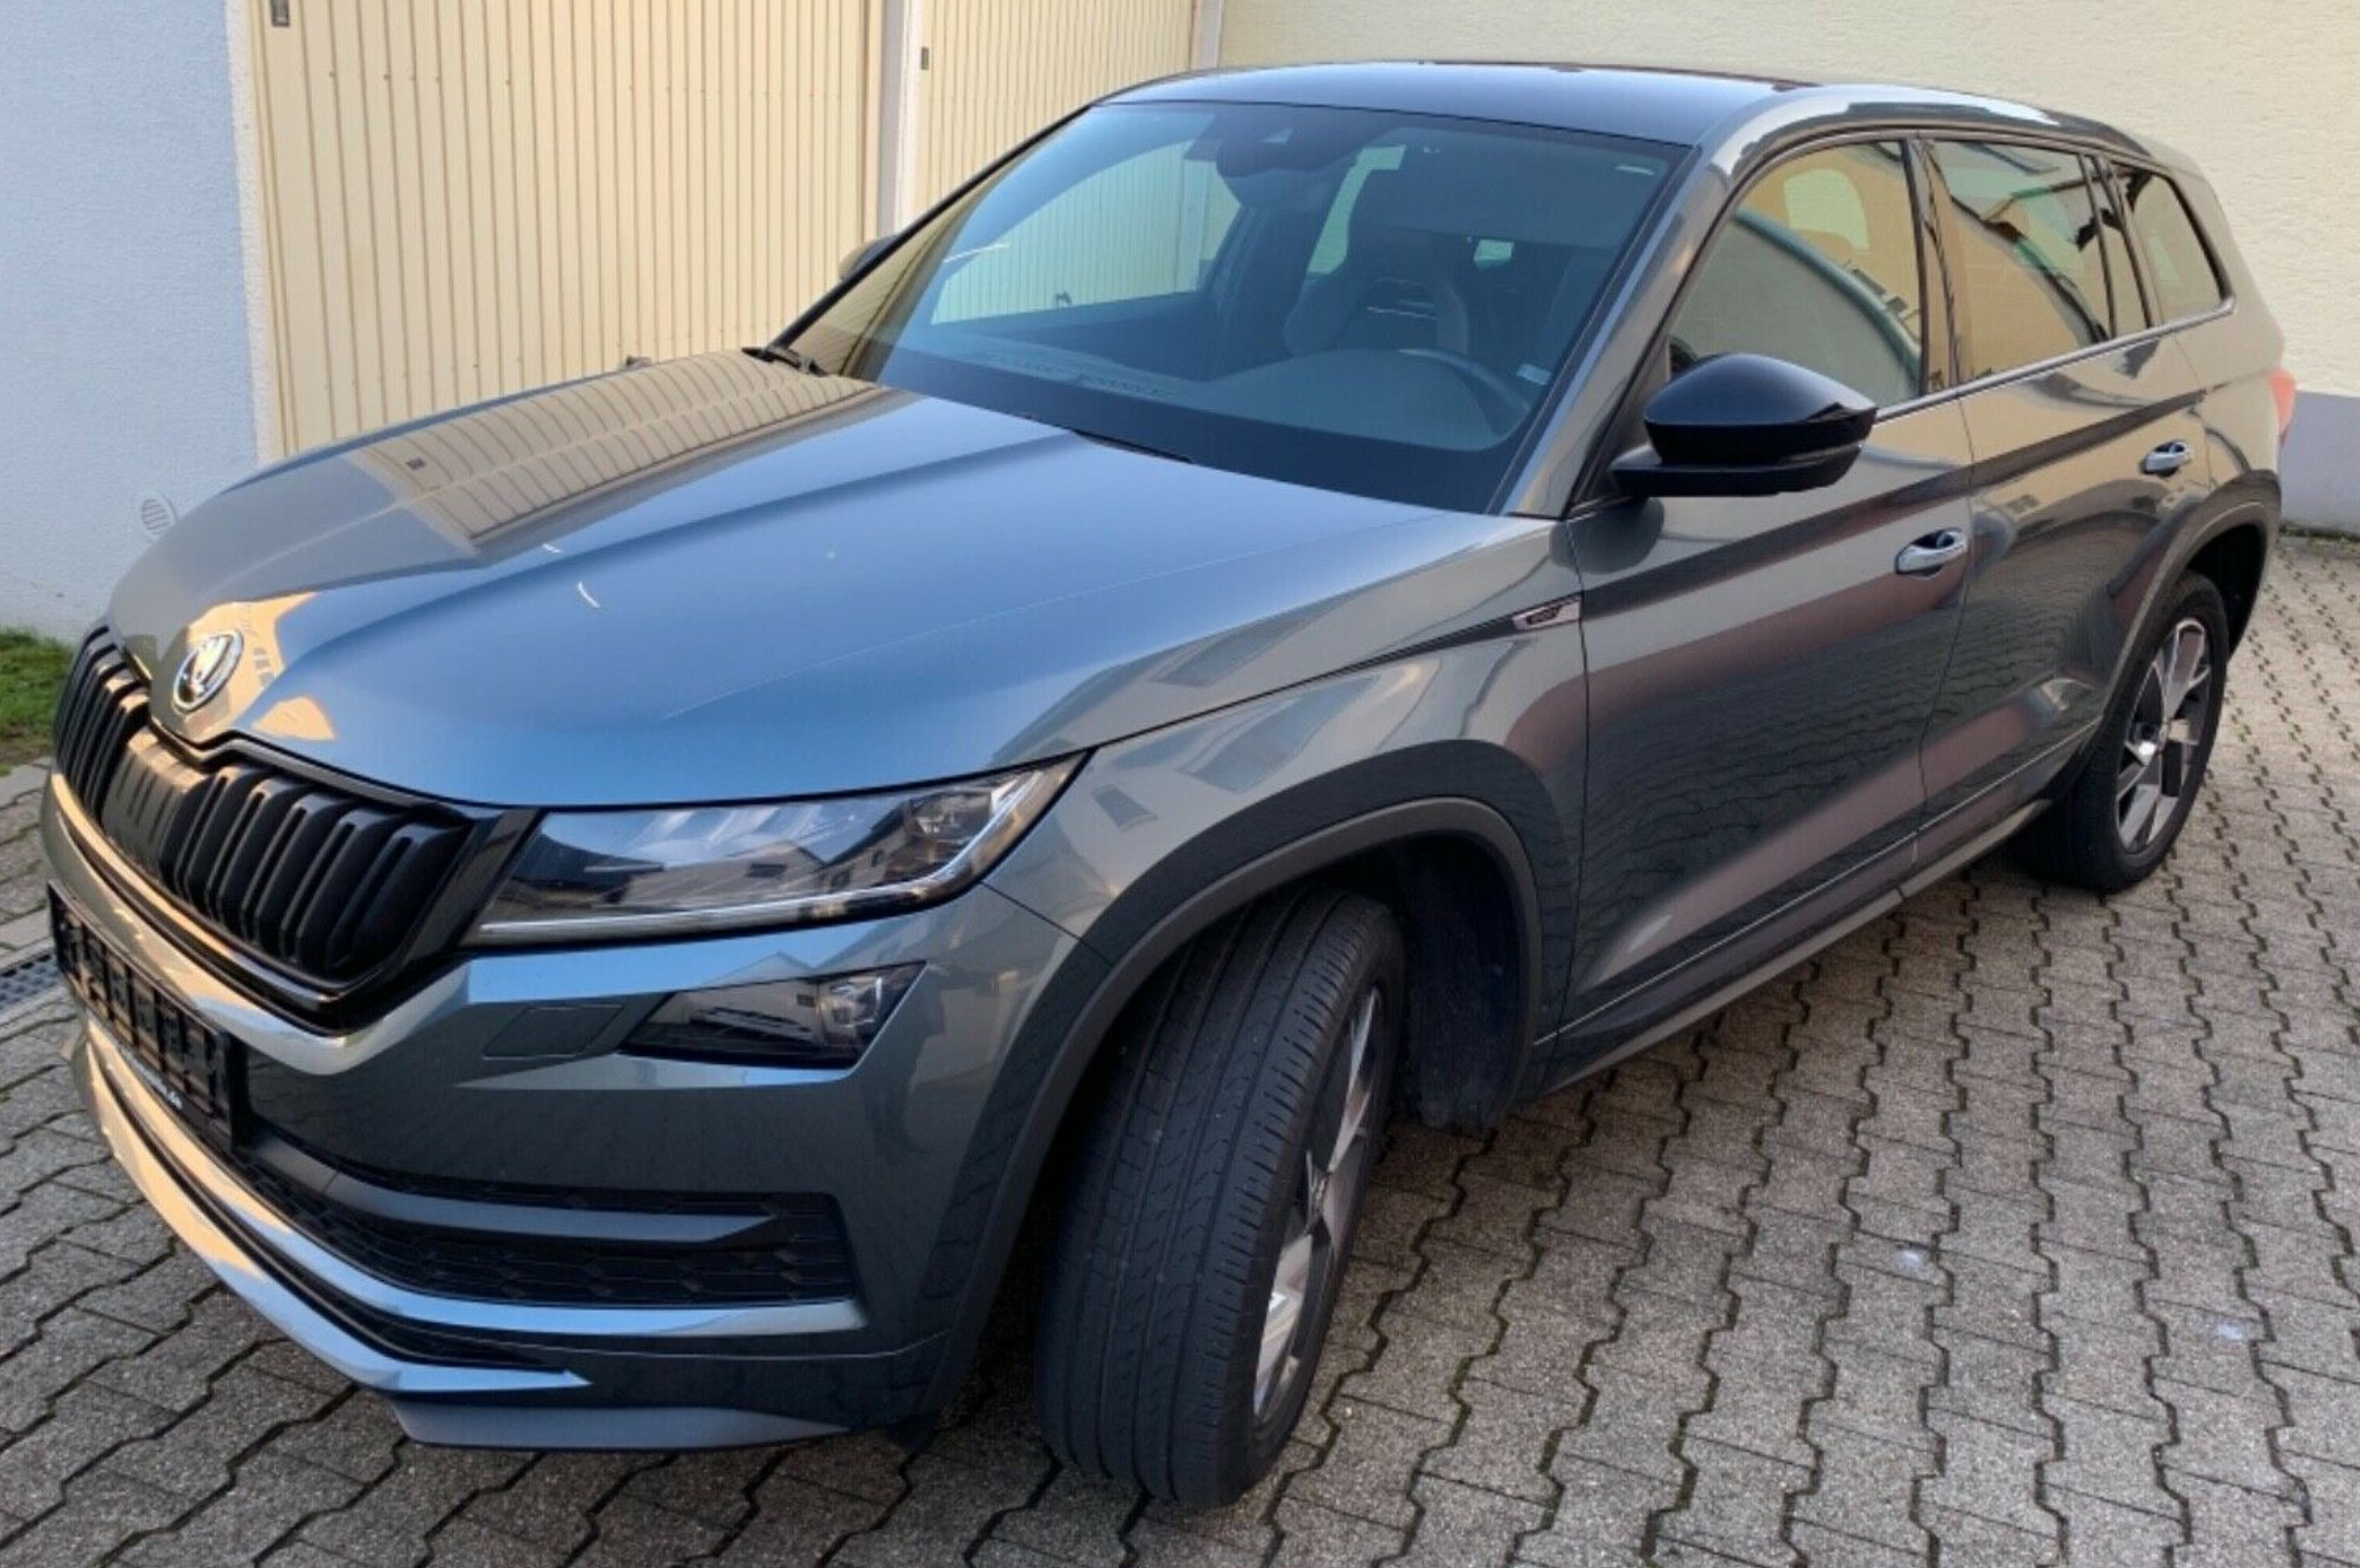
\includegraphics[width=0.9\columnwidth]{cars/skoda-kodiaq-4x4-2p0-tdi.png}

Skoda Kodiaq
\end{center}

\begin{itemize}
    \item LL/BJ: 83080/2018, 7-Sitzer $\rightarrow$ Laufzeit: 4 Jahre
    \item \href{https://suchen.mobile.de/fahrzeuge/details.html?action=parkItem&id=336544234}{Weblink}
    \item \emph{Gesch\"atzter} Spritpreis \"uber Haltedauer: 1.63 \euro{}/l
    \item Antrieb: Diesel, mit 192 PS
    \item Restwert nach Faustformel (Kaufpreis $\times$ 39.7\%): 11897.57 \euro{}
\end{itemize}

\begin{small}
\emph{Meinung Nataliya:} 0/10: 
        
\emph{Meinung Grzegorz:} 0/10: 
\end{small}

\pagebreak


\twocolumn

\section*{VW Touran, gebraucht, Benzin, Kredit}
\begin{center}
\includegraphics[width=0.5\textheight]{images1/vw-touran-g150kB7-boundaries_.png}
\null
\vspace{0.5cm}
\includegraphics[width=0.5\textheight]{images1/vw-touran-g150kB7-calc_df_.png}
\end{center}

\pagebreak
\begin{center}
\includegraphics[width=0.9\columnwidth]{cars/vw-touran-geb.png}

VW Touran
\end{center}

\begin{itemize}
    \item LL/BJ: 67640/2018, 7-Sitzer $\rightarrow$ Laufzeit: 4 Jahre
    \item \href{https://suchen.mobile.de/fahrzeuge/details.html?id=338082714}{Weblink}
    \item \emph{Gesch\"atzter} Spritpreis \"uber Haltedauer: 1.64 \euro{}/l
    \item Antrieb: Benzin, mit 150 PS
    \item Restwert nach Faustformel (Kaufpreis $\times$ 39.7\%): 9917.29 \euro{}
\end{itemize}

\begin{small}
\emph{Meinung Nataliya:} 0/10: 
        
\emph{Meinung Grzegorz:} 0/10: 
\end{small}

\pagebreak


\twocolumn

\section*{VW Touran, gebraucht, Benzin, Kredit}
\begin{center}
\includegraphics[width=0.5\textheight]{images1/vw-touran-g179kB7-boundaries_.png}
\null
\vspace{0.5cm}
\includegraphics[width=0.5\textheight]{images1/vw-touran-g179kB7-calc_df_.png}
\end{center}

\pagebreak
\begin{center}
\includegraphics[width=0.9\columnwidth]{cars/vw-touran-geb2.png}

VW Touran
\end{center}

\begin{itemize}
    \item LL/BJ: 53600/2018, 7-Sitzer $\rightarrow$ Laufzeit: 4 Jahre
    \item \href{https://suchen.mobile.de/fahrzeuge/details.html?id=337573342}{Weblink}
    \item \emph{Gesch\"atzter} Spritpreis \"uber Haltedauer: 1.64 \euro{}/l
    \item Antrieb: Benzin, mit 179 PS
    \item Restwert nach Faustformel (Kaufpreis $\times$ 39.7\%): 10234.77 \euro{}
\end{itemize}

\begin{small}
\emph{Meinung Nataliya:} 0/10: 
        
\emph{Meinung Grzegorz:} 0/10: 
\end{small}

\pagebreak


\twocolumn

\section*{VW Sharan, neu, Benzin, Kredit}
\begin{center}
\includegraphics[width=0.5\textheight]{images1/vw-sharan-n150kB7-boundaries_.png}
\null
\vspace{0.5cm}
\includegraphics[width=0.5\textheight]{images1/vw-sharan-n150kB7-calc_df_.png}
\end{center}

\pagebreak
\begin{center}
\includegraphics[width=0.9\columnwidth]{cars/vw-sharan.png}

VW Sharan
\end{center}

\begin{itemize}
    \item LL/BJ: 0/2022, 7-Sitzer $\rightarrow$ Laufzeit: 7 Jahre
    \item \href{https://www.volkswagen.de/de/konfigurator.html/__app/sharan/sharan/highline.app?buildabilityStatus-app=buildable&category-app=private&carlineId-app=31605&salesGroupId-app=32850&trimName-app=Highline&modelId-app=7N24GY%24GYOIYOI%24GYOUYOU&modelVersion-app=0&modelYear-app=2022&exteriorId-app=F14+0Q0Q&interiorId-app=F56+++++BY&options-app=GPF2PF2-GWBEWBE-GWG1WG1-GWH3WH3-GYOWYOW-MAHV1M6-MKSUKA2-MSSH4KF}{Weblink}
    \item \emph{Gesch\"atzter} Spritpreis \"uber Haltedauer: 1.64 \euro{}/l
    \item Antrieb: Benzin, mit 150 PS
    \item Restwert nach Faustformel (Kaufpreis $\times$ 19.8\%): 9654.05 \euro{}
\end{itemize}

\begin{small}
\emph{Meinung Nataliya:} 0/10: 
        
\emph{Meinung Grzegorz:} 0/10: 
\end{small}

\pagebreak


\twocolumn

\section*{VW Touran, neu, Benzin, Kredit}
\begin{center}
\includegraphics[width=0.5\textheight]{images1/vw-touran-n150kB7-boundaries_.png}
\null
\vspace{0.5cm}
\includegraphics[width=0.5\textheight]{images1/vw-touran-n150kB7-calc_df_.png}
\end{center}

\pagebreak
\begin{center}
\includegraphics[width=0.9\columnwidth]{cars/vw-touran-neu-benzin.png}

VW Touran
\end{center}

\begin{itemize}
    \item LL/BJ: 0/2022, 7-Sitzer $\rightarrow$ Laufzeit: 7 Jahre
    \item \href{https://www.volkswagen.de/de/konfigurator.html/__app/touran/touran/highline.app?buildabilityStatus-app=buildable&category-app=private&carlineId-app=31000&salesGroupId-app=32600&trimName-app=Highline&modelId-app=5T14PZ%24GYORYOR&modelVersion-app=2&modelYear-app=2022&exteriorId-app=F14+0Q0Q&interiorId-app=F56+++++BG&options-app=GWBGWBG-GPG3PG3-MAHV1M6-GPF9PF9-GRBDRBD-MKSUKA1-MSSH4KF-GP19P19-MVTV9IJ-GWQ1WQ1}{Weblink}
    \item \emph{Gesch\"atzter} Spritpreis \"uber Haltedauer: 1.64 \euro{}/l
    \item Antrieb: Benzin, mit 150 PS
    \item Restwert nach Faustformel (Kaufpreis $\times$ 19.8\%): 7708.28 \euro{}
\end{itemize}

\begin{small}
\emph{Meinung Nataliya:} 0/10: 
        
\emph{Meinung Grzegorz:} 0/10: 
\end{small}

\pagebreak


\twocolumn

\section*{VW Touran, neu, Diesel, Kredit}
\begin{center}
\includegraphics[width=0.5\textheight]{images1/vw-touran-n150kD7-boundaries_.png}
\null
\vspace{0.5cm}
\includegraphics[width=0.5\textheight]{images1/vw-touran-n150kD7-calc_df_.png}
\end{center}

\pagebreak
\begin{center}
\includegraphics[width=0.9\columnwidth]{cars/vw-touran-neu-benzin.png}

VW Touran
\end{center}

\begin{itemize}
    \item LL/BJ: 0/2022, 7-Sitzer $\rightarrow$ Laufzeit: 7 Jahre
    \item \href{https://www.volkswagen.de/de/konfigurator.html/__app/touran/touran/highline.app?buildabilityStatus-app=buildable&category-app=private&carlineId-app=31000&salesGroupId-app=32600&trimName-app=Highline&modelId-app=5T146Z%24GYORYOR&modelVersion-app=1&modelYear-app=2022&exteriorId-app=F14+0Q0Q&interiorId-app=F56+++++BG&options-app=GWBGWBG-GPG3PG3-MAHV1M6-GPF9PF9-GRBDRBD-MKSUKA1-MSSH4KF-GP19P19-MVTV9IJ-GWQ1WQ1}{Weblink}
    \item \emph{Gesch\"atzter} Spritpreis \"uber Haltedauer: 1.63 \euro{}/l
    \item Antrieb: Diesel, mit 150 PS
    \item Restwert nach Faustformel (Kaufpreis $\times$ 19.8\%): 8304.16 \euro{}
\end{itemize}

\begin{small}
\emph{Meinung Nataliya:} 0/10: 
        
\emph{Meinung Grzegorz:} 0/10: 
\end{small}

\pagebreak


\twocolumn

\section*{VW Tiguan Allspace, neu, Diesel, Kredit}
\begin{center}
\includegraphics[width=0.5\textheight]{images1/vw-tiguan-allspace-n200kD7-boundaries_.png}
\null
\vspace{0.5cm}
\includegraphics[width=0.5\textheight]{images1/vw-tiguan-allspace-n200kD7-calc_df_.png}
\end{center}

\pagebreak
\begin{center}
\includegraphics[width=0.9\columnwidth]{cars/vw-tiguan-diesel.png}

VW Tiguan Allspace
\end{center}

\begin{itemize}
    \item LL/BJ: 0/2022, 7-Sitzer $\rightarrow$ Laufzeit: 7 Jahre
    \item \href{https://www.volkswagen.de/de/konfigurator.html/__app/der-neue-tiguan-allspace/der-tiguan-allspace---standardmodelle/elegance.app?buildabilityStatus-app=buildable&category-app=private&carlineId-app=31160&salesGroupId-app=32700&trimName-app=Elegance&modelId-app=BJ247T%24GYORYOR&modelVersion-app=2&modelYear-app=2022&exteriorId-app=F14+0Q0Q&interiorId-app=F56+++++BG&options-app=GWBAWBA-GPG4PG4-MAHV1M6-GPFCPFC-GRBDRBD-MKSUKA2}{Weblink}
    \item \emph{Gesch\"atzter} Spritpreis \"uber Haltedauer: 1.63 \euro{}/l
    \item Antrieb: Diesel, mit 200 PS
    \item Restwert nach Faustformel (Kaufpreis $\times$ 19.8\%): 9414.30 \euro{}
\end{itemize}

\begin{small}
\emph{Meinung Nataliya:} 0/10: 
        
\emph{Meinung Grzegorz:} 0/10: 
\end{small}

\pagebreak


\twocolumn

\section*{VW Tiguan Allspace, neu, Benzin, Kredit}
\begin{center}
\includegraphics[width=0.5\textheight]{images1/vw-tiguan-allspace-n190kB7-boundaries_.png}
\null
\vspace{0.5cm}
\includegraphics[width=0.5\textheight]{images1/vw-tiguan-allspace-n190kB7-calc_df_.png}
\end{center}

\pagebreak
\begin{center}
\includegraphics[width=0.9\columnwidth]{cars/vw-tiguan-diesel.png}

VW Tiguan Allspace
\end{center}

\begin{itemize}
    \item LL/BJ: 0/2022, 7-Sitzer $\rightarrow$ Laufzeit: 7 Jahre
    \item \href{https://www.volkswagen.de/de/konfigurator.html/__app/der-neue-tiguan-allspace/der-tiguan-allspace---standardmodelle/elegance.app?buildabilityStatus-app=buildable&category-app=private&carlineId-app=31160&salesGroupId-app=32700&trimName-app=Elegance&modelId-app=BJ247T%24GYORYOR&modelVersion-app=2&modelYear-app=2022&exteriorId-app=F14+0Q0Q&interiorId-app=F56+++++BG&options-app=GWBAWBA-GPG4PG4-MAHV1M6-GPFCPFC-GRBDRBD-MKSUKA2}{Weblink}
    \item \emph{Gesch\"atzter} Spritpreis \"uber Haltedauer: 1.64 \euro{}/l
    \item Antrieb: Benzin, mit 190 PS
    \item Restwert nach Faustformel (Kaufpreis $\times$ 19.8\%): 8809.70 \euro{}
\end{itemize}

\begin{small}
\emph{Meinung Nataliya:} 0/10: 
        
\emph{Meinung Grzegorz:} 0/10: 
\end{small}

\pagebreak



\pagebreak

\onecolumn
\begin{figure}
\centering
Vergleich der monatlichen Kosten bei \euro{} 15000.00 Anzahlung bei Kreditfinanzierung und \euro{} 3000.00 bei Leasing.

Gesch\"atzer Kraftstoffpreis: 1.64 \euro{}/l Benzin, 1.63 \euro{}/l Diesel bzw. 0.31 \euro{}/kWh


\vspace{1em}
\includegraphics[width=0.95\columnwidth]{images1/overview1.png}
\end{figure}
\vfill 



\end{document}
